% =================
% Bots
% =================
\subsection{Bot/Shell}

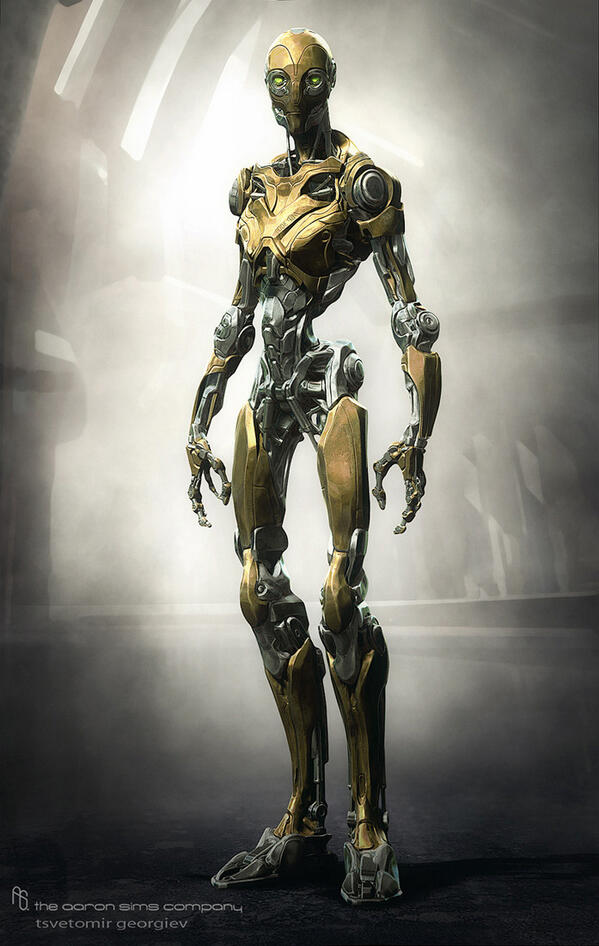
\includegraphics[width=\linewidth]{BEzZuPdCEAAgcr8}

A common sight on any technologically-advanced society is the large number of Bots and machines performing menial yet necessary labour. Most of these machines are limited to a singular purpose and have a "weak AI". But technology has advanced far enough that some robots can be programmed to display human-like cognitive abilities. These Bots are considered to have "strong AI", and are used for highly specialised and complex work.

On the other end of the spectrum are individuals who have made the transition from organic to mechanical. These individuals, known as Ghosts, have chosen to digitise their conciousness and memory and upload themselves into artificial bodies known as Shells. Many in society believe that these digitised conciousnesses have lost their basic "humanity", and are indistinguishable from normal AI.

All Bot and Shell characters have the following traits:
\begin{standardtable}{\linewidth}{sb}
  \textbf{Artificial} & Organic races often mistrust and misunderstand Bots and Shells. -2 to Charisma when dealing with races other than their own. Organics will generally prefer to deal with an organic "master", and are wary of any machine that claims it is operating independently\\
  \textbf{Construct} & Add +2 to recover from being Shaken, do not suffer wound modifiers, and are immune to poison and disease. They cannot Heal naturally, and require the Repair skill to remove wounds (use like the Healing skill).\\
  \textbf{Recharge} & If you cannot access a power source at least once a day, suffer one point of Fatigue each day until incapacitated. The day after that, you go "off-line" and must be revivied with a Repair roll and a four-hour charge. This replaces the need for food and water.\\
\end{standardtable}

In addition, as a digital conciousness you are able to swap your physical "body" to suit the task at hand. However, purchasing new bodies is extremely expensive and your chassis model will only be able to improve a little bit before it hits it's technological limits. Please note that while playing a Bot or Ghost character offers lots of flexibility, your progress may stall when you hit your chassis' experience limit and you cannot afford an upgrade.

All of your characters Attributes, Skills and Edges are linked to a particular chassis you own. You cannot carry over any attributes, skills or edges across to a new chassis. Your character retains all of their memories and personality, and your Cortical Stack may be recoverable from the wreckage of your chassis (although all attributes, skills and edges will be lost to the chassis). If the Cortical Stack is damaged or lost, you can recover from a back-up (without all of the new memories).

It also should be noted that it is highly illegal to run multiple copies of yourself throughout United Systems space and most Independent systems.

The following applies to each chassis you own:
\begin{standardtable}{\linewidth}{sb}
  \textbf{All Shiny} & Your chassis has it's own rank (Novice, Seasoned, Veteran, Heroic, Legendary). Your character must be of the same rank to pilot the chassis. The chassis can never improve it's rank. When creating the chassis, purchase advancements up till the rank of the chassis\\
  \textbf{Bugs} & All chassis have some sort of manufactoring or programming problem. Select one Major OR two Minor hindrances that make sense for your chassis. Do not gain any character creation points\\
  \textbf{Deus Ex Machina} & Your chassis gains experience points seperately to your character. It gains experience while you are operating the chassis (it also gains experience if someone else operates the chassis). Gained experience points can be used to buy advancements, up until the chassis reaches the next rank (max. 4 advancements)\\
  \textbf{Disorientation} & You will experience disorientation as you get used to your new chassis. The settling period usually occurs over a few days (4d4 OR at the GM's discretion), after which you will be totally fluent in the capabilities of your new body. If you attempt to do any task during the disorientation period, apply a -2 penalty
\end{standardtable}

\begin{paperbox}{Hacking} 
Hacking and reprogramming a Bot is a very complex task. It will generally require the Hacker to access a physical IO port (most computer and electronic systems guard against remote entry), which is best accessed if the Bot is incapacitated. Then the Hacker needs to open the IO port (Hacker's Repair vs Bot's Toughness), and then break the software Firewalls (Hacker's Security opposed by the Bot's Spirit).
\end{paperbox}

\begin{commentbox}{Becoming the System} 
Since you are a digital consciousness, there is nothing stopping you from inhabiting other computer or cybernetic systems. There are just a few cavaets:
  \begin{itemize}
    \item \textbf{Hardware}: Not all computer systems have enough memory, processing power or disk storage to hold and operate a digital conciousness. In these cases it is better to interact with the system through a standard interface port instead\\
    \item \textbf{Firewalls}: Unless you have been allowed to inhabit the computer system, there is likely to be multiple security systems in place to lock out and destroy intruders. Use the Hacking rules to determine if you can bypass the Firewalls\\
    \item \textbf{Limited Sensors}: Most computer system do not even bother with audio visual input, relying on a user to type in commands through a terminal or keyboard. You could lose sense of the outside world while inhabiting the computer system\\
    \item \textbf{Illegal}: Across most jurisdictions it is illegal for an AI or Ghost to co-inhabit on a single computer with other AIs or programs. This is because most co-habited computers ended up with one AI "murdering" all other programs and AI so that they could have uncontested access to the system hardware. For this reason, all computer hardware (including Bots) must be blank before uploading an AI or program, and (in the case of swapping) the hardware left behind must be blanked upon exiting\\
    \item \textbf{Disorientation}: It is always a disorientating experience when being uploaded to a new environment. Follow the rules outlined in Disorientation section for the chassis
  \end{itemize}
\end{commentbox}
